\documentclass{beamer}
\usetheme{Darmstadt}
\usecolortheme{beaver}
\usepackage{booktabs}
\usepackage{hyperref}

\usepackage[utf8]{inputenc}
\usepackage{graphicx}
\graphicspath{ {./images/} }

%Information to be included in the title page:
\title{Sample title}
\author{Brandon Hosley}
\institute{University of Illinois - Springfield}
\date{\today}

\begin{document}
\frame{\titlepage}

\begin{frame}{Overview}
\tableofcontents
\end{frame}

\section[Q1.1]{Q1A: What is a Na\"{i}ve-Bayes classifier?}

\begin{frame}{Na\"{i}ve-Bayes}
	\begin{itemize}[<+->]
		\item Based on Bayes' Theorem
		\item By comparing a series of known probabilities one may infer the probability of an associated outcome/event/attribute
		\item Na\"{i}ve means that the known variables are being treated as independent
	\end{itemize}
	
	\onslide<1->{
		\begin{block}{Bayes' Theorem} $P(A|B)=\frac{P(B|A)P(A)}{P(B)}$ \end{block}
	}
	\onslide<2->{
		\begin{exampleblock}{Bayes' Theorem Generalized} 
			$P(C_k|x_1,\ldots,x_n)=P(C_k)\prod_{i=1}^{n} \frac{P(x_i|C_k)}{P(x_i)}$ 
		\end{exampleblock}
	}
\end{frame}
\begin{frame}{Na\"{i}ve-Bayes classification}
	\begin{itemize}[<+->]
		\item From training data we can build our classifier
		\item From the data set we can estimate $P(x)$ and $P(C_k)$
			for all of our attributes \\
			If these values are not similar in the test set it warns of a poor sample
		\item $P(x_i|C_k)$ is determined from the sample data and is the resource intensive aspect of developing a classifier in this method.
	\end{itemize}
	\begin{exampleblock}{Bayes' Theorem Generalized} 
		$P(C_k|x_1,\ldots,x_n)=P(C_k)\prod_{i=1}^{n} \frac{P(x_i|C_k)}{P(x_i)}$ 
	\end{exampleblock}
\end{frame}

\section[Q1.2]{Q1B: What are the evaluation metrics for classification in machine learning?}

\section[Q2]{Q2: Hastie and Tibshirani Summary}

\begin{frame}{Tibshirani Lecture: Classification}
\begin{itemize}
	\item<1-> Linear Regression
	\begin{itemize}
		\item<1-> Simple approximation method
		\item<1-> Great for estimating slope of data
		\item<1-> From this one may generate confidence interval
	\end{itemize}
	\item<2> Hypothesis Testing
	\begin{itemize}
		\item<2> Testing against a null hypothesis
		\item<2>[] $H_0$ : No relationship between $X$ and $Y$.
		\item<2> Testing for the probability of independent variable distribution 
	\end{itemize}
\end{itemize}
%\only<1>{\includegraphics[width=0.75\linewidth]{ConfidenceIntervals}}
%\only<2>{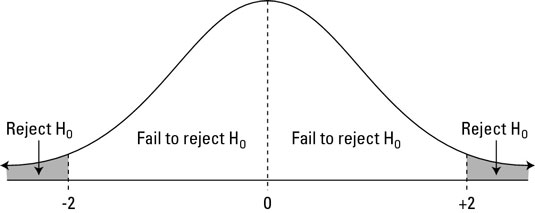
\includegraphics[width=0.75\linewidth]{nullHypothesis}}
\end{frame}

\end{document}
